%%%%%%%%%%%%%%%%%%%%%%%%%%%%%%%%%%%%%%%%%%%%%%%%%%%%%%%%%%%%%%%%%%%%%%%%%%%
% This is LaTeX file for Homework Assignment 1 of CS460
% Author: Shuo Yang
%%%%%%%%%%%%%%%%%%%%%%%%%%%%%%%%%%%%%%%%%%%%%%%%%%%%%%%%%%%%%%%%%%%%%%%%%%%

\documentclass[11pt]{article}
\usepackage{amsmath,amssymb,epsfig,graphics,hyperref,amsthm,mathtools}
\DeclarePairedDelimiter\ceil{\lceil}{\rceil}
\DeclarePairedDelimiter\floor{\lfloor}{\rfloor}

\hypersetup{colorlinks=true}

\setlength{\textwidth}{7in}
\setlength{\topmargin}{-0.575in}
\setlength{\textheight}{9.25in}
\setlength{\oddsidemargin}{-.25in}
\setlength{\evensidemargin}{-.25in}

\reversemarginpar
\setlength{\marginparsep}{-15mm}

\newcommand{\rmv}[1]{}
\newcommand{\bemph}[1]{{\bfseries\itshape#1}}
\newcommand{\N}{\mathbb{N}}
\newcommand{\Z}{\mathbb{Z}}
\newcommand{\imply}{\to}
\newcommand{\bic}{\leftrightarrow}

% Some user defined strings for the homework assignment
%
\def\CourseCode{CS460}
\def\AssignmentNo{1}
\def\DateHandedOut{Spring, 2016}
\def\Author{Shuo Yang}

\begin{document}

\noindent

\CourseCode \hfill \DateHandedOut

\begin{center}
Homework \#\AssignmentNo\\
TA: \Author\\
\end{center}

% A horizontal split line
\hrule\smallskip

% Enumerate through all questions.
\begin{enumerate}
\item Database approach is different with the file-based approach in
  three ways:
  \begin{enumerate}
  \item Unlike file-based approach, where the structure of data is
    embedded in the application programs, database approach decouples the
    structure of data from the application programs, thus providing
    data-program independence. In database approach, the structure of
    data is held in system catalog (or data dictionary) and programs
    can share data.
  \item Database approach also reduces unnecessary data redundancy
    which is often the case in the file-base approach.
  \end{enumerate}

\item
  \begin{tabular}{| l | p{3.5cm} | p{5cm} | p{5.5cm} |}
    \hline
    & Point of view & Functions & Relationship with other levels
    \\ \hline
    External level & User's view of data & Let users access data that
    is customized to their needs & Interfaces with conceptual level to
    provide logical independence\\ \hline
    Conceptual level & Community view of database, seen by DBA &
    Describes the logical structure of the entire database, but is
    independent of any storage considerations & Interfaces with external
    level to support external views and interfaces with internal level
    to provide physical data independence \\ \hline
    Internal level & Physical representation of the database &
    Describes how data is stored in the database & Interfaces with
    conceptual level to provide physical data independence \\ \hline
  \end {tabular}

\item The three-tier client-server architecture maps naturally to
  the Web with a web browser acting as a thin client, an application
  server handling user requests and a database server managing data
  access. This architecture has better modularity (easier to modify
  or replace one tier without affecting the others), better load
  balancing (with the separation of core business logic from the
  database functions) compared to the two-tier client-server
  architecture for traditional DBMSs.

\item MySQL supports client-server architecture because it was
  designed to operate in a networking environment where multiple users
  can simultaneously connect to the database to make requests. In
  MySQL package, \emph{mysqld} is the server program that manages
  database and handles client requests, \emph{mysql} is the client
  program that connects to \emph{mysqld} to access the database.

\item Mathematical relations are based on set theory.\\
  Let $D_1,D_2, \cdots D_n$ be $n$ sets(domains). Their Cartesian
  product is defined as:
  \begin{equation}
    D_1 \times D_2 \times \cdots \times D_n = \{(d_1,d_2,\cdots,d_n) |
    d_1 \in D_1, d_2 \in D_2, \cdots d_n \in D_n\}
  \end{equation}
  A mathematical relation on the $n$ sets is defined as any set of
  $n$-tuples from this Cartesian product.

  Now let $A_1,A_2,\cdots,A_n$ be attributes with values drawing from
  the domains $D_1,D_2, \cdots D_n$. Then the set
  $\{A_1:D_1,A_2:D_2,\cdots,A_n:D_n\}$ is a relation schema. In
  relational model, a relation defined by the relation schema is a set
  of mapping from the attribute names to their corresponding
  domains. Thus, a relation $R$ is a set of $n$-tuples:
  \begin{equation}
    R = \{(A_1:d_1,A_2:d_2,\cdots,A_n:d_n) | d_1 \in D_1, d_2 \in D_2,
    \cdots d_n \in D_n\}
  \end{equation}
  In this way, we can think of a relation in the relational model as
  any subset of the Cartesian product of the domains of the
  attributes.

\item 
  The primary key is the candidate key that is selected to identify
  tuples uniquely within a relation.\\
  A foreign key is an attribute or set of attributes within one
  relation that matches the candidate key of some (possibly the same)
  relation.

  For example, consider the following relations:\\\\
  \textbf{Student}(\underline{UANetID}, firstName, lastName, CSID)\\
  \textbf{Grade}(\underline{CSID}, \underline{Assignment\#}, score)\\
  \textbf{Employee}(\underline{SSN}, firstName, lastName, superSSN)\\

  where \emph{CSID} in the \textbf{Student} relation is a candidate
  key. Thus \emph{CSID} in the \textbf{Grade} table is a foreign key
  refers to the candidate key CSID in the \textbf{Student}
  relation. \emph{superSSN}(supervisor's SSN) is a foreign key refers
  to the primary key \emph{SSN} in the same relation.

\item 
  A relationship type is a set of associations between one or more
  participating entity types.

  \begin{enumerate}
  \item Unary relationship (recursive relationship):\\
    Employee \emph{supervises} employee
  \item Binary relationship:\\
    Doctor \emph{works for} Hospital
  \item Ternary relationship:\\
    Client \emph{sees} Doctor \emph{at} Hospital
  \end{enumerate}

\item 
  The relationship \textbf{Newspaper} \emph{Advertises}
  \textbf{PropertyForRent} consists of two attributes:
  \underline{dateAdvert} (representing the date the advert took 
  place) and \underline{cost} (representing the cost of the advert).

\item ER diagram is shown below:
  \begin{center}
    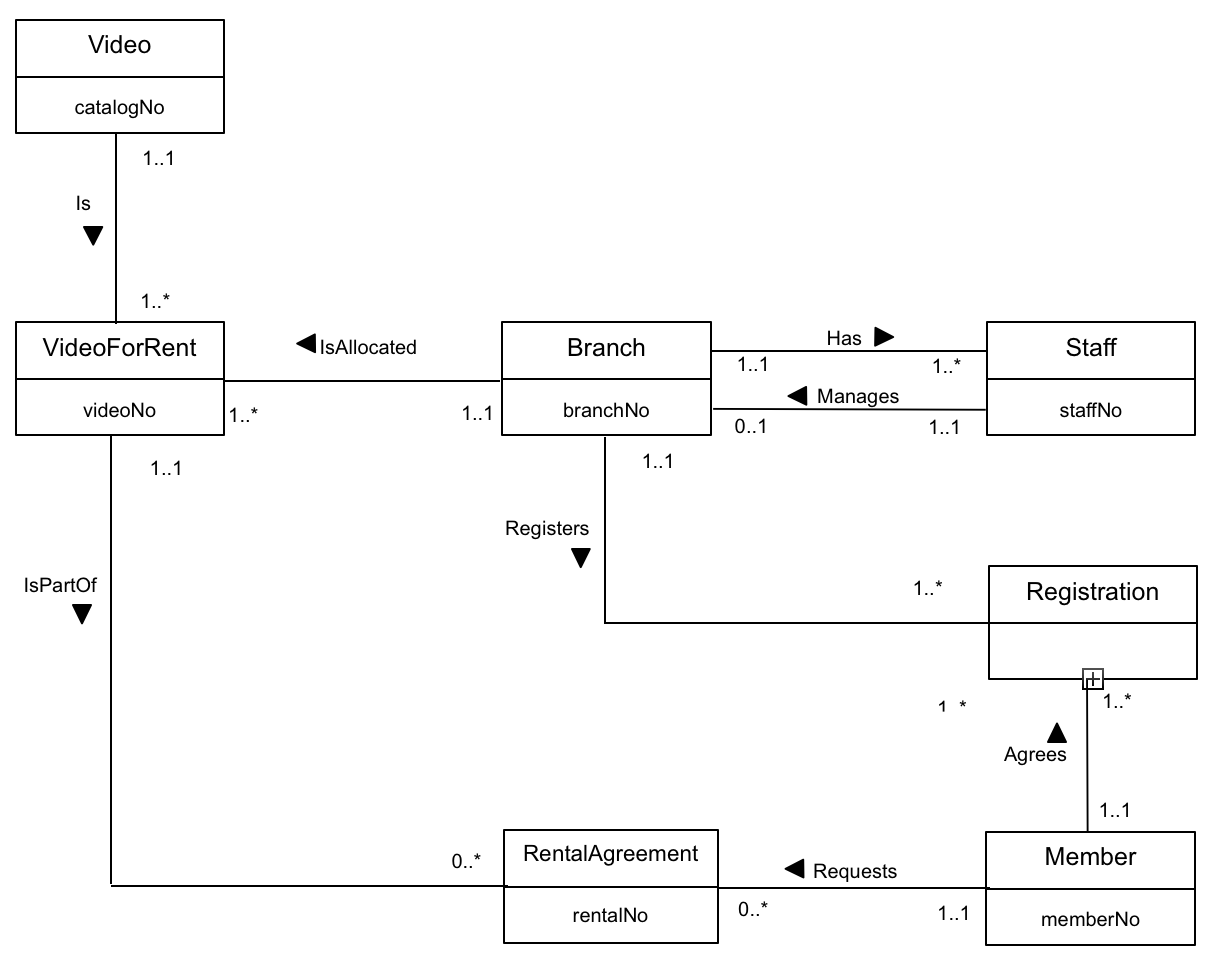
\includegraphics[width=12cm,height=10cm]{./Q12-12.png}
  \end{center}

\item
  Consider Manager as a specialization of the Staff entity. This would
  move the Manages relationship from Staff to the Manager
  subclass. However, the attributes for both entities would be the
  same and there would, therefore, seem to be no obvious advantage to
  introducing the Manager specialization.

\item
  \begin{enumerate}
  \item The system fails if either one of the four hard drives
    fails. Put it in another way, the system works only if all the
    four hard drives do not fail. The probability of the system not
    fail is:
    \begin{align}
      P_{nf} &= (1-0.015)^2 \times (1-0.03)^2\\
      &\approx 0.913\\
      &= 91.3\%
    \end{align}

    Therefore the probability of failure of the system is:
    \begin{align}
      P_{f} &= 1 - P_{nf}\\
      &= 0.087\\
      &= 8.7\%
    \end{align}

  \item In order to exceed a 50\% failure rate, we need to satisfy the
    following condition:
    \begin{align}
      P_{f} &= 1 - P_{nf}\\
      &= 1 - ((1-0.015)^{n} \times (1-0.03)^{n})\\
      &> 50\%
    \end{align}
    When $n=15$, $P_f = 49.5\%$. When $n=16$, $P_f = 51.8\%$. Thus
    there must be at least 32 hard drives the RAID system would have
    to exceed a $50\%$ failure rate.
  \end{enumerate}

\item Dynamic hashing index structure is shown below:
  \begin{center}
    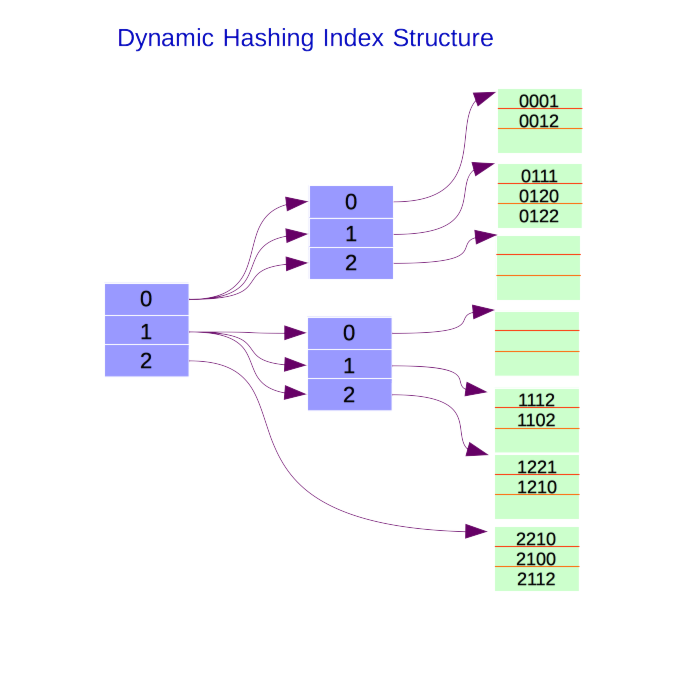
\includegraphics[width=10cm,height=10cm]{cs460-hw1-Q12.png}
  \end{center}

\item
  \begin{enumerate}
  \item Insertion process of $B^+$ tree is shown below:
    \begin{center}
    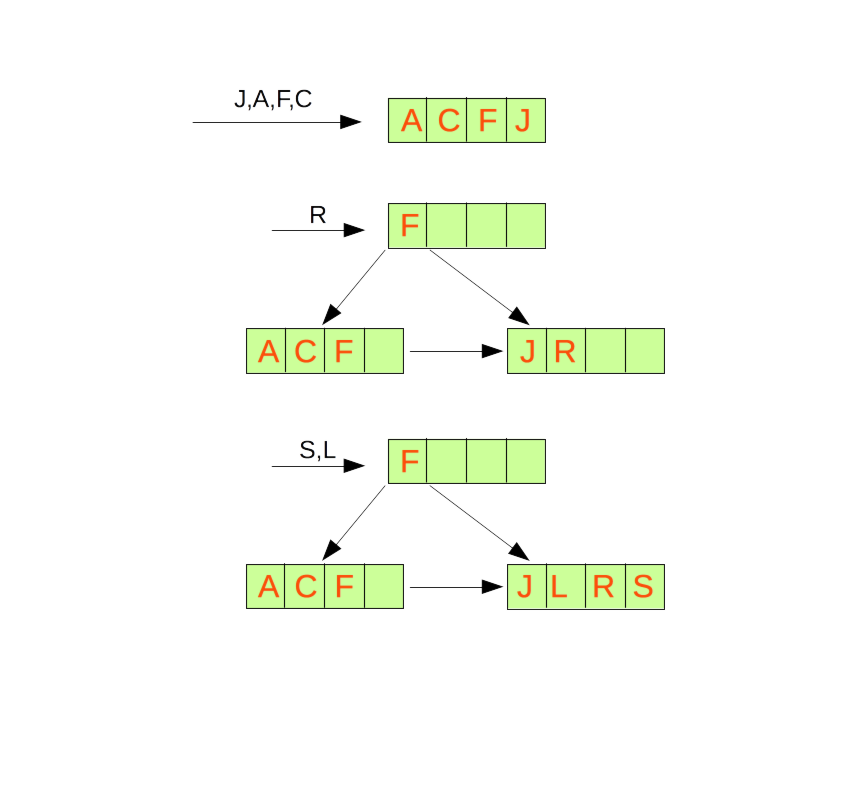
\includegraphics[width=10cm,height=10cm]{cs460-hw1-Q13-a.png}
    \end{center}

  \item Deletion process of $B^+$ tree is shown below:
    \begin{center}
      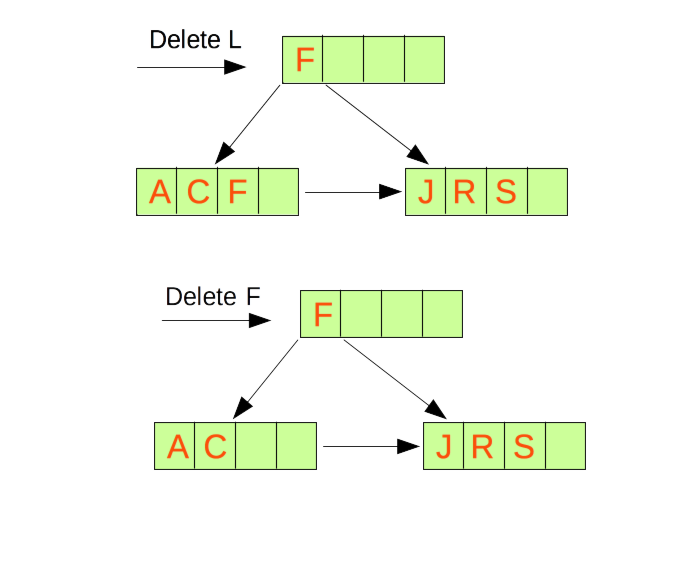
\includegraphics[width=8cm,height=8cm]{cs460-hw1-Q13-b.png}
    \end{center}
  \end{enumerate}

\end{enumerate}
\end{document}
